% IMPORTANT
% when clicking 'Typeset' the main file should always be open

\documentclass[11pt]{report}	% document class, beginning of every .tex
\usepackage[english, german]{babel}	% language setting
\usepackage{geometry}             % See geometry.pdf to learn the layout options. There are lots.
\geometry{a4paper}                   % ... or a4paper or a5paper or ... 
%\usepackage[parfill]{parskip}   % Activate to begin paragraphs with an empty line rather than an indentt
\usepackage{xifthen}
\usepackage{xstring}			% to check content of strings in xifthen
\usepackage{graphicx}
\usepackage{tabularx}
\usepackage[usenames,dvipsnames,table]{xcolor}
\usepackage{amssymb}
\usepackage{epstopdf}
\usepackage[utf8]{inputenc}
\usepackage{hyperref}
\usepackage{fancyhdr}
\usepackage{float}
%\usepackage{natbib}
\usepackage{url}

\newcommand{\titleofthesis}{Erweiterung des WYSIWYG Texteditors "Trix" für Barrierefreiheit}
\newcommand{\department}{Medientechnik} % Replace by your department

\newcommand{\firstauthor}{Halil Bahar}
\newcommand{\firstauthorclass}{5AHITM}
\newcommand{\secondauthor}{Sonja Cao}
\newcommand{\secondauthorclass}{5AHITM}

\newcommand{\duedateen}{April 21, 2021} % due date in english format
\newcommand{\duedatede}{21. April 2021} % due date in german format
\newcommand{\supervisor}{Prof. Mag. Ing. Dr. Thomas Stütz}
\newcommand{\projectpartner}{Fabasoft Software GmbH} % Set basic data (author, title, etc.) of your thesis
\IfStrEq*{\languagename}{english}
	{
		\newcommand{\dalabel}{Diploma Thesis}
		\newcommand{\submittedlabel}{Submitted by}
		\newcommand{\datelabel}{Date}
		\newcommand{\duedatevalue}{\duedateen}
		\newcommand{\supervisorlabel}{Supervisor}
		\newcommand{\projectpartnerlabel}{Project Partner}
	}
	{
		\newcommand{\dalabel}{Diplomarbeit}
		\newcommand{\submittedlabel}{Eingereicht von}
		\newcommand{\datelabel}{Datum}
		\newcommand{\duedatevalue}{\duedatede}
		\newcommand{\supervisorlabel}{Betreuer}
		\newcommand{\projectpartnerlabel}{Projektpartner}
	}
 % This file should not really be touched

\begin{document}
\rhead{
\includegraphics[scale=.9]{images/Logo.png}}
\cfoot{}
\begin{titlepage}
\thispagestyle{fancy}

\begin{center}

\vspace*{8em}

{\LARGE \dalabel}

\vspace{2em}

{\large Höhere Technische Bundeslehranstalt Leonding \\[.5em]
Abteilung für \department}

%\vspace{8em}
\vspace*{\fill}

{\Huge \titleofthesis}
\end{center}

%\vspace{8em}
\vspace*{\fill}

\begin{tabular}{ll}
\ifthenelse{\isundefined{\firstauthor}}{}{\submittedlabel: & {\bf \firstauthor, \firstauthorclass}}
\ifthenelse{\isundefined{\secondauthor}}{}{ \\[.5em] & {\bf \secondauthor, \secondauthorclass}}
\ifthenelse{\isundefined{\thirdauthor}}{}{ \\[.5em] & {\bf \thirdauthor, \thirdauthorclass}}
\ifthenelse{\isundefined{\fourthauthor}}{}{ \\[.5em] & {\bf \fourthauthor, \fourthauthorclass}}
 \\[.5em]
\datelabel: & {\bf \duedatevalue} \\[.5em]

\supervisorlabel: & {\bf \supervisor} \\[.5em]

\ifthenelse{\isundefined{\projectpartner}}{}{\projectpartnerlabel: & {\bf \projectpartner}}
\end{tabular}
\end{titlepage}
 % Should not be necessary to touch this file
\section*{Declaration of Academic Honesty} % * ... section numbering
Hereby, I declare that I have composed the presented paper independently on my own and without any other resources than the ones indicated. All thoughts taken directly or indirectly from external sources are properly denoted as such.

This paper has neither been previously submitted to another authority nor has it been published yet. \\[1em]
Leonding, \duedateen \\[5em]
\ifthenelse{\isundefined{\firstauthor}}{}{\firstauthor}
\ifthenelse{\isundefined{\secondauthor}}{}{\kern-1ex, \secondauthor}
\ifthenelse{\isundefined{\thirdauthor}}{}{\kern-1ex, \thirdauthor}
\ifthenelse{\isundefined{\fourthauthor}}{}{\kern-1ex, \fourthauthor} \\[5em]

\begin{otherlanguage}{german}
\section*{Eidesstattliche Erklärung}
Hiermit erkläre ich an Eides statt, dass ich die vorgelegte Diplomarbeit selbstständig und ohne Benutzung anderer als der angegebenen Hilfsmittel angefertigt habe. Gedanken, die aus fremden Quellen direkt oder indirekt übernommen wurden, sind als solche gekennzeichnet.

Die Arbeit wurde bisher in gleicher oder ähnlicher Weise keiner anderen Prüfungsbehörde vorgelegt und auch noch nicht veröffentlicht. \\[1em]
Leonding, am \duedatede \\[5em]
\ifthenelse{\isundefined{\firstauthor}}{}{\firstauthor}
\ifthenelse{\isundefined{\secondauthor}}{}{\kern-1ex, \secondauthor}
\ifthenelse{\isundefined{\thirdauthor}}{}{\kern-1ex, \thirdauthor}
\ifthenelse{\isundefined{\fourthauthor}}{}{\kern-1ex, \fourthauthor} \\[5em]
\end{otherlanguage}

\section*{Gender Declaration} % * ... section numbering
In this diploma thesis the language form of the generic masculine is used for reasons of better readability. All personal designations are therefore to be understood as gender-neutral.

\begin{otherlanguage}{german}
\section*{Gender Erklärung}
Aus Gründen der besseren Lesbarkeit wird in dieser Diplomarbeit die Sprachform des generischen Maskulinums verwendet. Alle personenbezogenen Bezeichnungen sind somit geschlechtsneutral zu verstehen.
\end{otherlanguage}

\begin{otherlanguage}{english}
\begin{abstract} % environment 'abstract'
In the course of the diploma thesis of Halil Bahar and Sonja Cao an extension for the open source What You See Is What You Get (WYSIWYG) text editor Trix from the company Basecamp is being developed for the client Fabasoft Software GmbH. The previous text editor of the Fabasoft Cloud no longer meets the desired requirements and Trix is still unsuitable in terms of accessibility for people with disabilities. The extension is therefore intended to be used in products of Fabasoft and to meet the criteria of WCAG 2.1, making it accessible with screen readers and the keyboard to enable all users to write and format texts without barriers.

\end{abstract}
\end{otherlanguage}

\begin{otherlanguage}{german}
\begin{abstract}
Im Zuge der Diplomarbeit von Halil Bahar und Sonja Cao wird der Open Source What You See Is What You Get (WYSIWYG) Texteditor namens Trix vom Unternehmen Basecamp für den Auftraggeber Fabasoft Software GmbH erweitert. Der bisherige Texteditor der Fabasoft Cloud entspricht nicht mehr den gewünschten Anforderungen und Trix ist hinsichtlich der Accessibility für Menschen mit Beeinträchtigungen noch ungeeignet. Die Erweiterung soll daher einen Einsatz in Fabasoft Produkten ermöglichen sowie die Kriterien der WCAG 2.1 erfüllen und so mit Screenreadern sowie Tastatur zugänglich sein, um allen Benutzern die Möglichkeit zu geben, Texte barrierefrei zu verfassen und zu formatieren.

\end{abstract}
\end{otherlanguage}

\section*{Danksagung}
Wir möchten uns bei allen Personen bedanken, die uns bei unserer Arbeit unterstützt haben, um ein erfolgreiches Ergebnis zu liefern:

%\begin{itemize}
%	\item 
%\end{itemize}

 % Declaration of Academic Honesty, Abstracts, Acknowledgments, 

\tableofcontents

% it is better to create a new file for every chapter
\chapter{Einleitung}
\section{Ausgangssituation}
Die Fa. Fabasoft ist ein mittelständisches Unternehmen im Zentralraum Oberösterreichs. Zum Geschäftsmodell zählen die Entwicklung und der Vertrieb von Softwareprodukten, die vor allem für die Bereiche Enterprise Search, Wissensmanagement, digitale Geschäftsprozesse und unternehmensübergreifende Zusammenarbeit in der Cloud konzipiert sind. Kunden sind private und öffentliche Auftraggeber, insbesondere des E-Governments, und Wirtschaftsunternehmen, die hohe Sicherheitsanforderungen stellen und hauptsächlich im deutschsprachigen Raum beheimatet sind. Ein Grundkonzept der Fabasoft Cloud ist Barrierefreiheit. Dieses Produkt wurde im Oktober 2019 als erste Web-Applikation von der Österreichischen Computer Gesellschaft mit dem WACA-Zertifikat (Web Accessibility Certificate Austria \cite{waca_zertifikate_2020}) in der Stufe Silber ausgezeichnet.

\section{Ist-Zustand}
Ein Grundkonzept der Fabasoft Cloud ist Barrierefreiheit, Ziel ist es, dass die Benutzeroberfläche von allen Menschen, unabhängig ihrer Behinderungen, bedient werden kann.
Oftmals wird in Softwareprodukten der Fa. Fabasoft die Eingabe von einfachen, formatierten Texten gefordert, die in einem WYSIWYG (What You See Is What You Get) Rich Text Editor erfasst werden. 
Übersetzt bedeutet ``What You See Is What You Get`` so viel wie ``Was du siehst, ist das, was du bekommst``. Der Text in einem WYSIWYG Editor wird bei der Ausgabe des Dokuments also genau so angezeigt, wie er bei seiner Bearbeitung aussieht.\\
Ein Beispiel für solch einen Editor ist ``Trix``. Er ist ein Open Source WYSIWYG Texteditor vom Unternehmen Basecamp, den Machern von Ruby on Rails, und wurde von den beiden Entwicklern Sam Stephenson und Javan Makhmali der Community auf GitHub \cite{basecamp_trix_2013} zugänglich gemacht. Mithilfe dieses Editors können Nachrichten, Kommentare, Artikel, Listen und vieles mehr verfasst werden. Es besitzt ein selbst entwickeltes Document Object Model (DOM), das neben den gängigen JavaScript Events ebenso auf selbst definierte Events hört und eingebettete Anhänge unterstützt.

\subsection{Document Object Model}
\begin{figure}[H]
\begin{center}
	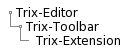
\includegraphics[scale=1]{images/dom_tree.png}
\end{center}
	\caption{Zusammenhang zwischen Trix und der Erweiterung}
\end{figure}

\section{Motivation}
Der bisher integrierte Browser-UI-Control in Fabasoft Softwareprodukten weist einige Nachteile auf. Der sogenannte ``CKEditor`` \cite{ckeditor_v4_2020} in der Version 4 verliert seinen Long Term Support (LTS) im Jahr 2023. Dieser wird von der Version 5 \cite{ckeditor_v5_2020} abgelöst. Da die neue Version eine neue Lizenz mit sich bringt, ist dieser Texteditor in den Produkten nicht mehr weiterhin verwendbar. Der Grund dafür ist, dass die neue Lizenz unter den Bedingungen der GNU General Public License Version 2 or later (GPLv2) steht und der Sourcecode auf Nachfrage freigegeben werden muss. Das entspricht nicht der Philosophie der Firma. Darum wird der Editor durch ein alternatives Produkt abgelöst. Durch eine erste Analyse hat sich herausgestellt, dass sich der Texteditor {\em{Trix}} als Ersatz eignet. Allerdings ist dieser nicht barrierefrei.

\subsection{Gleichstellung von Menschen mit Behinderungen}
In der Gesellschaft und im Alltag machen Menschen mit Behinderungen oftmals mit kleineren oder größeren Benachteiligungen Bekanntschaft. Global haben etwa 15 Prozent der Weltbevölkerung eine Behinderung, wobei die rund eine Milliarden Kinder und Erwachsenen assistive Technologien, wie beispielsweise Rollstühle oder Hörgeräte, benötigen. International hat jedes Land eine eigene Definition für den Begriff, weshalb die WHO (World Health Organisation, vgl. \cite{who_disability_2011}) diesen nur grob beschreiben kann. Sie geht dabei immer von drei Punkten aus:

\begin{itemize}
    \item \textbf{Impairment (dt. Schädigung)} bezeichnet jede Anomalie oder jeden Verlust der anatomischen, psychischen oder physiologischen Funktionen und Strukturen des menschlichen Körpers.
    \item \textbf{Disability (dt. Beeinträchtigung)} bezeichnet jeden Mangel oder jede Einschränkung der Fähigkeiten infolge einer Beeinträchtigung, wodurch eine von der Gesellschaft als normal oder in diesem Bereich betrachtete Tätigkeit nicht ausgeübt werden kann.
    \item \textbf{Handicap (dt. Behinderung)} bezeichnet den Nachteil einer Person aufgrund einer Schädigung oder Beeinträchtigung. Eine Behinderung steht im Zusammenhang mit einem Problem mit einer Struktur oder eines Organes des Körpers.
\end{itemize}

\mbox{}\\Grundsätzlich wird eine Behinderung in Österreich als dauerhafte Auswirkung einer körperlichen, geistigen oder psychischen Beeinträchtigung oder Beeinträchtigung der Sinnesfunktionen bezeichnet. Diese überschreitet einen Zeitraum von sechs Monaten und erschwert die Teilhabe in der Gesellschaft. Damit die Benachteiligung von Behinderten möglichst flächendeckend beseitigt wird, können diesbezügliche Gesetze auf der Webseite des Rechtsinformationssystems des Bundes (RIS) abgerufen werden:

\begin{itemize}
    \item Das Bundesgesetz über die Gleichstellung von Menschen mit Behinderungen (Bundes-Behindertengleichstellungsgesetz - BGStG, vgl. \cite{ris_bgstg_2020}) zur Regelung der Diskriminierung im täglichen Leben.
    \item Das Behinderteneinstellungsgesetz (BEinstG, vgl. \cite{ris_beinstg_2020}) zur Regelung der Diskriminierung in der Arbeitswelt.
    \item Das Bundesgesetz vom 17. Mai 1990 über die Beratung, Betreuung und besondere Hilfe für behinderte Menschen (Bundesbehindertengesetz - BBG, vgl. \cite{ris_bbg_2020}) zur Regelung der Aufgaben und Befugnisse des Behindertenanwalts.
\end{itemize}

Die Fassung des BGStG besagt, dass das Ziel die Beseitigung der Diskriminierung von Menschen mit Behinderungen sei, um diese gleichberechtigt am Leben in der Gesellschaft teilhaben zu lassen und eine selbstbestimmte Lebensführung zu gewährleisten. Der Diskriminierungsschutz gilt somit für diejenigen, die körperlich, geistig, psychisch behindert oder sinnesbehindert sind, ebenso für ihre Angehörigen. Es ist nicht erlaubt jemanden unmittelbar oder mittelbar zu diskriminieren.

\paragraph{Definition: Diskriminierung}\mbox{}\\
Wird eine Person aufgrund ihrer Behinderung in bestimmten Situationen oder gegenüber anderen anders behandelt, so liegt eine unmittelbare Diskriminierung vor. Eine mittelbare Diskriminierung hingegen liegt genau dann vor, wenn neutrale Vorschriften, Kriterien, Verfahren oder Merkmale gestalteter Lebensbereiche den Anschein erwecken, Menschen mit Behinderungen gegenüber anderen auf jegliche Art und Weise zu benachteiligen.\\
Zu diesen Benachteiligungen gehören: 
\begin{itemize}
    \item Barrieren
    \item eine weniger günstige Behandlung
    \item Diskriminierungsaufforderungen
    \item und Belästigung aufgrund einer Behinderung
\end{itemize}

\paragraph{Arten von Behinderungen}\mbox{}\\
Grundsätzlich lassen sich Behinderungen in sechs Kategorien einteilen:

\begin{itemize}
    \item \textbf{Körperliche Behinderungen} kommen am häufigsten vor und nehmen nicht selten mit dem Alter zu. Bezeichnet werden damit starke physische Einschränkungen, die auf eine Dysfunktion oder Schädigung der Stütz- und Bewegungsorgane zurückgeführt werden.
    \item \textbf{Geistige Behinderungen} sind fortwährende, deutlich über dem Durchschnitt liegende Einschränkungen der kognitiven Fähigkeiten und kommen am zweithäufigsten vor. Zu diesen kognitiven Fähigkeiten zählen die Wahrnehmung, die Aufmerksamkeit, das Denken und das Lernen ebenso wie die Erinnerung, die Motivation und die Konzentration.
    \item \textbf{Sinnesbehinderungen} umfassen alle Seh- sowie Hörbehinderungen wie Fehlsichtigkeit, Blindheit, Schwerhörigkeit, Gehörlosigkeit und Taubblindheit.
    \item \textbf{Sprachbehinderungen} oder anders formuliert Störungen des Redeflusses, des Spracherwerbs, des Sprechens und der Stimme bezeichnet all jene Menschen, die nicht fähig sind ihre Muttersprache im entsprechenden Alter schriftlich oder mündlich zu beherrschen.
    \item \textbf{Psychische Behinderungen} umfassen die Beeinflussung des Denkens, Fühlens und Handelns von Menschen. Das heißt wiederum, dass es Abgrenzungen zwischen Verhalten und Erleben gibt.
\end{itemize}

\section{Barrierefreiheit im Web}
\subsection{Definition: Web-Zugänglichkeit}
Web-Zugänglichkeit oder im Englischen auch ``Web Accessibility'' bezeichnet, dass alle Menschen auf dem bestmöglichen Weg Zugang zu Information oder Dienstleistung im Internet haben. Ziel ist es, Websites und jegliche mobile Anwendungen für alle Nutzerinnen und Nutzer, vor allem auch diejenigen mit Behinderungen, besser zugänglich und somit barrierefrei zu gestalten. In der heutigen Gesellschaft ist das Internet mit all seinen verfügbaren Leistungen kaum noch wegzudenken. Zahlreiche Dienstleistungen wie etwa Onlinebanking, elektronische Dienste von Instituten und Institutionen, Onlineshop und viele mehr gehören dazu.\\
Das Web-Zugänglichkeits-Gesetz (WZG, vlg. \cite{ris_wzg_2020}) umfasst alle rechtlichen Grundlagen zur Erreichung dieses Ziels. Insbesondere der Bund und alle mit ihm in Zusammenhang stehende Einrichtungen sind dazu verpflichtet barrierefreie Dienstleistungen bereitzustellen. Hierzu gibt es bestimmte Anforderungen:

\begin{itemize}
    \item Wahrnehmbarkeit
    \item Bedienbarkeit
    \item Verständlichkeit
    \item Robustheit
\end{itemize}

\mbox{}\\Des Weiteren wurde ein zeitlicher Anwendungsbereich festgelegt, in dem alle Websites und mobile Anwendungen des Bundes barrierefrei sein müssen:

\begin{itemize}
    \item Neue Websites nach dem 23. September 2018 ab dem 23. September 2019
    \item Alte Websites vor dem 23. September 2018 ab dem 23. September 2020
    \item Alle mobilen Anwendungen ab dem 23. Juni 2021
\end{itemize}

\mbox{}\\Damit diese Dienstleistungen fortlaufend zugänglich sind, müssen die oben genannten Anforderungen regelmäßig überprüft werden. Grundsätzlich hat jede Nutzerin und jeder Nutzer das Recht dazu, sich über Mängel bei Nichteinhaltung der Barrierefreiheit zu beschweren, die dann, wenn sie berechtigt sind, beseitigt werden müssen. 

\section{Aufgabenstellung}
Im Rahmen dieser Diplomarbeit ist der Texteditor {\em{Trix}} so erweitert worden, dass er den Ansprüchen für die Produkte der Fa. Fabasoft gerecht wird, mit dem Ziel, dass er von allen Personen einfach und ohne Probleme bedient werden kann. Insbesondere wurden die Kriterien des WCAG 2.1 (Web Content Accessibility Guidelines \cite{wcag_2_1_2018}) erfüllt sowie eine Bedienung mit Screenreadern und vollständig mit Tastatur ermöglicht worden.

\section{Zielsetzung}
Ziel dieser Arbeit war es, den Mitarbeiten und Kunden von Fabasoft die Verwendung eines Texteditors weiterhin zu ermöglichen sowie den bis dahin verwendeten Editor abzulösen. Des Weiteren sind mindestens dessen bisher verfügbaren Funktionalitäten bereitgestellt und alle Kriterien des WCAG 2.1 erfüllt.

\subsection{Systemarchitektur}
% Trix ohne Erweiterung - Wie verwendet? Produkt beschreiben
\begin{figure}[H]
\begin{center}
	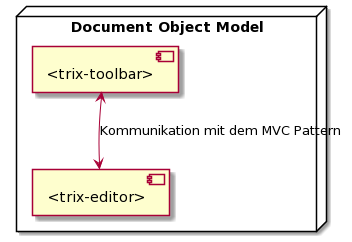
\includegraphics[scale=.6]{images/trix_components.png}
\end{center}
	\caption{Kommunikation zwischen der Toolbar und dem Editor ohne der Erweiterung}
\end{figure}

% Trix mit Erweiterung - Art von Formatvorlage, DOM Manipulation, evtl. Jenkinsfile
\begin{figure}[H]
\begin{center}
	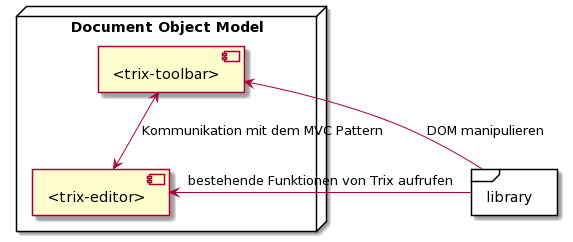
\includegraphics[scale=.6]{images/trix-extension_components.png}
\end{center}
	\caption{Schnittstellen zwischen dem Texteditor und der Bibliothek für die Erweiterung - Durch die DOM Manipulation können zusätzlich Buttons erstellt werden, die für Trix nicht vorgesehen waren (vgl. Trix-Extension Buttons \ref{subsec:buttons})}
\end{figure}

\section{Sollzustand}
% Erweiterung genauer beschreiben

\subsection{Funktionale Anforderungen}
Für diese Diplomarbeit sind keine funktionalen Anforderungen definiert.

\subsection{Nichtfunktionale Anforderungen}

\begin{itemize}
	\item Aufsetzen eines npm-basierten Build-Prozesses mit allen notwendigen Artefakten in das Fabasoft npm-Repository.
	\item Aufbau einer Unit-Test-Infrastruktur mit einer Line-Coverage von mindestens 70 Prozent.
	\item Einpflegen der entsprechenden Änderungen zur Erfüllung der Kriterien des WCAG 2.1.
	\item Vollständige Bedienung über eine Tastatur und einen Screenreader.
	\item Einpflegen eines High-Level-APIs, um die Instanzierung und Parametrierung aus dem Fabasoft UI möglichst simpel zu gestalten.
	\item Schlussendliche Integration in die Softwareprodukte der Fa. Fabasoft.
\end{itemize}

\section{Projektablauf und Produkt}
\subsection{Projektablauf}
Im ersten Schritt ist das GitHub Repository des Texteditors Trix geforkt worden, um die notwendigen Änderungen zur Erreichung der Barrierefreiheit einzupflegen. Allerdings sind die Entwickler, die auch die gleichzeitigen Betreuer des Editors sind, bezüglich der Issues und der Pull Requests, sehr inaktiv. Daraufhin wurde eine eigene Erweiterung geschrieben, die unabhängig vom Sourcecode von Trix ist. Das bedeutet nun, dass kein Pull Request erstellt werden musste und dennoch eine barrierefreie Bedienung möglich ist.\\
Der nächste Schritt beinhaltet den korrekten Export der bestehenden formatierten Textinhalte in der Fabasoft Cloud. Damit keine zusätzlichen Zeilenumbrüche hinzugefügt und gewisse HTML Elemente unterstützt und nicht übersprungen werden, sind eine Reihe von Funktionalitäten in Trix selbst und mithilfe von JavaScript Prototypes überschrieben worden. Bei Bedarf können diese Überschreibungen ignoriert werden.

\subsection{Produkt}
Mithilfe der Erweiterung ist es möglich, den Texteditor über die Tastatur zu bedienen und somit visuelle Elemente, wie etwa Buttons, zum Formattieren des Textes zu erreichen. 
\chapter{Ausgewählte Technologien}
% languages, libraries, IDEs and tools
\section{Git und GitLab}

\subsection{Versionskontrollsystem}
Oftmals arbeitet ein Entwickler oder ein Entwicklerteam an einem Softwareprojekt, um entweder Fehler zu beheben oder neue Funktionalitäten hinzuzufügen. Hierbei werden Änderungen am Quellcode durchgeführt, die regelmäßig gesichert werden müssen. Diese Änderungen können in manchen Fällen auch dazu führen, dass etwas anderes im Code nicht mehr so funktioniert wie es sollte. Dann werden weitere Änderungen gemacht, um wieder einen lauffähigen Stand herzustellen, jedoch kann es passieren, dass plötzlich gar nichts mehr funktioniert.

\mbox{}\\Abhilfe für dieses Problem bietet ein Versionskontrollsystem, auch als VCS (Version Control System, vgl. \cite{vcs_2019}) bezeichnet, das Änderungen in der Projektentwicklung festhält. Dadurch ist es möglich zu einem späteren beliebigen Zeitpunkt auf ältere Versionen des Systems zurückzugreifen, den aktuellen Code mit früheren Versionen zu vergleichen oder Bugfixes zu implementieren. Arbeiten mehrere Entwickler an denselben Dateien im Quellcode, so kann mitverfolgt werden, welche Person welche Änderungen gemacht hat. Ein Projekt, das mit einem VCS verwaltet wird, wird Repository genannt. Ein Repository kann als eine Art Datenbank mit allen Änderungen betrachtet werden, die die History repräsentieren. Diese Änderungen sind ein markierter Stand, ein sogenannter Commit, in der Projektentwicklung und werden als Working Copy gespeichert, die einer Kopie des gesamten Projektes entspricht. Ein Commit kann als Schnappschuss oder als kleiner Meilenstein betrachtet werden. Er beinhaltet neben der Working Copy einen Zeitstempel und eine Nachricht, die aussagt, was sich seit dem letzten Commit geändert hat. Die Entwicklungsarbeiten können dabei in mehreren Entwicklungszweigen (engl. Branches) erfolgen. Eine Abspaltung eines Projektes wird hingegen als Fork bezeichnet.

\mbox{}\\Es gibt drei Arten von Version Control Systems:

\begin{itemize}
	\item \textbf{Lokal:} Lokale Versionskontrollsysteme funktionieren nur auf einem Rechner und versionieren eine einzige Datei. Insbesondere in Büroanwendungen kommen Tools wie Revision Control System (RCS) oder Source Code Control System (SCCS) zum Einsatz. Das Dokument speichert  dabei jede Version in seiner eigenen Datei.
	
	\begin{figure}[H]
	\begin{center}
		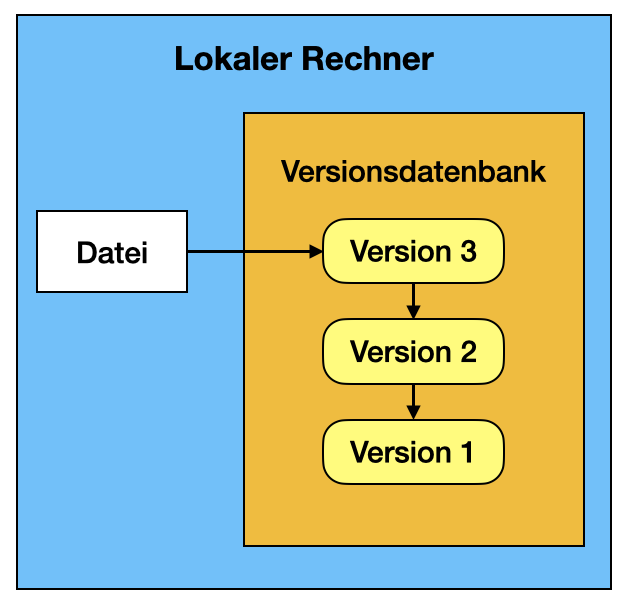
\includegraphics[scale=.65]{images/local_vcs.png}
	\end{center}
		\caption{Lokales Versionskontrollsystem}
	\end{figure}
	
	\item \textbf{Zentral:} Bei einem zentralisierten Versionskontrollsystem gibt es ein Respository, das sich mehrere 		Entwickler in einem Netzwerk miteinander teilen. Es handelt sich hierbei um ein Client-Server-System, das 		von zahlreichen kommerziellen Anbietern verwendet wird. Durch das Concurrent Versions System (CVS) 			wurde dieses Konzept berühmt, aber durch Subversion (SVN) neu implementiert.
	
	\begin{figure}[H]
	\begin{center}
		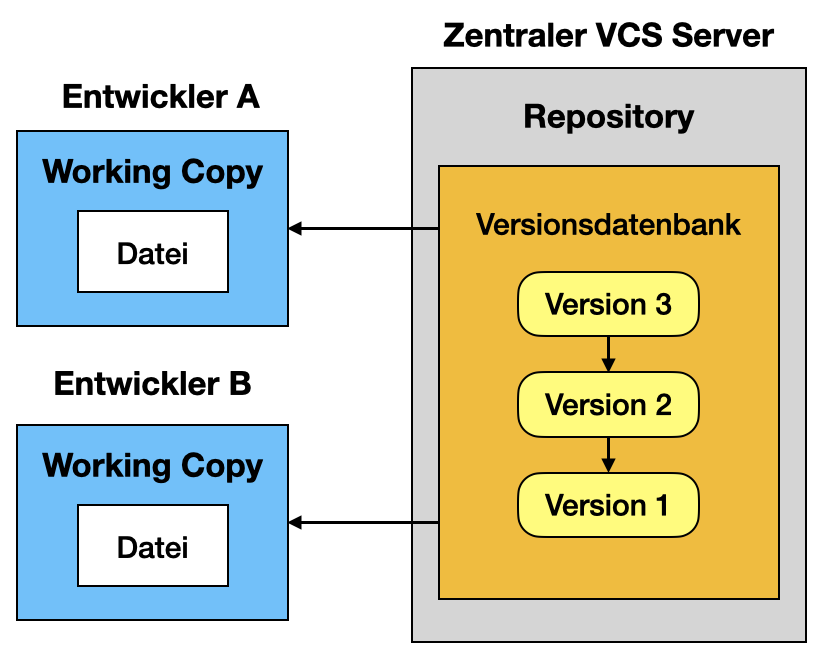
\includegraphics[scale=.65]{images/central_vcs.png}
	\end{center}
		\caption{Zentralisiertes Versionskontrollsystem}
	\end{figure}
	
	\item \textbf{Verteiltes VCS:} Im Gegensatz zum zentralisierten VCS existiert beim verteilten Versionskontrollsystem 		kein zentrales Repository. Jeder am Projekt tätige Entwickler verfügt über ein eigenes Repository, das er mit 		anderen Repositories abgleichen kann. Auch hier ist die History klar ersichtlich. Der einzige Unterschied zu 		den beiden anderen Versionskontrollsystemen ist der, dass Änderungen hier am lokalen Rechner erfolgen 		können. Eine Verbindung mit dem Server ist nicht notwendig.
	
	\begin{figure}[H]
	\begin{center}
		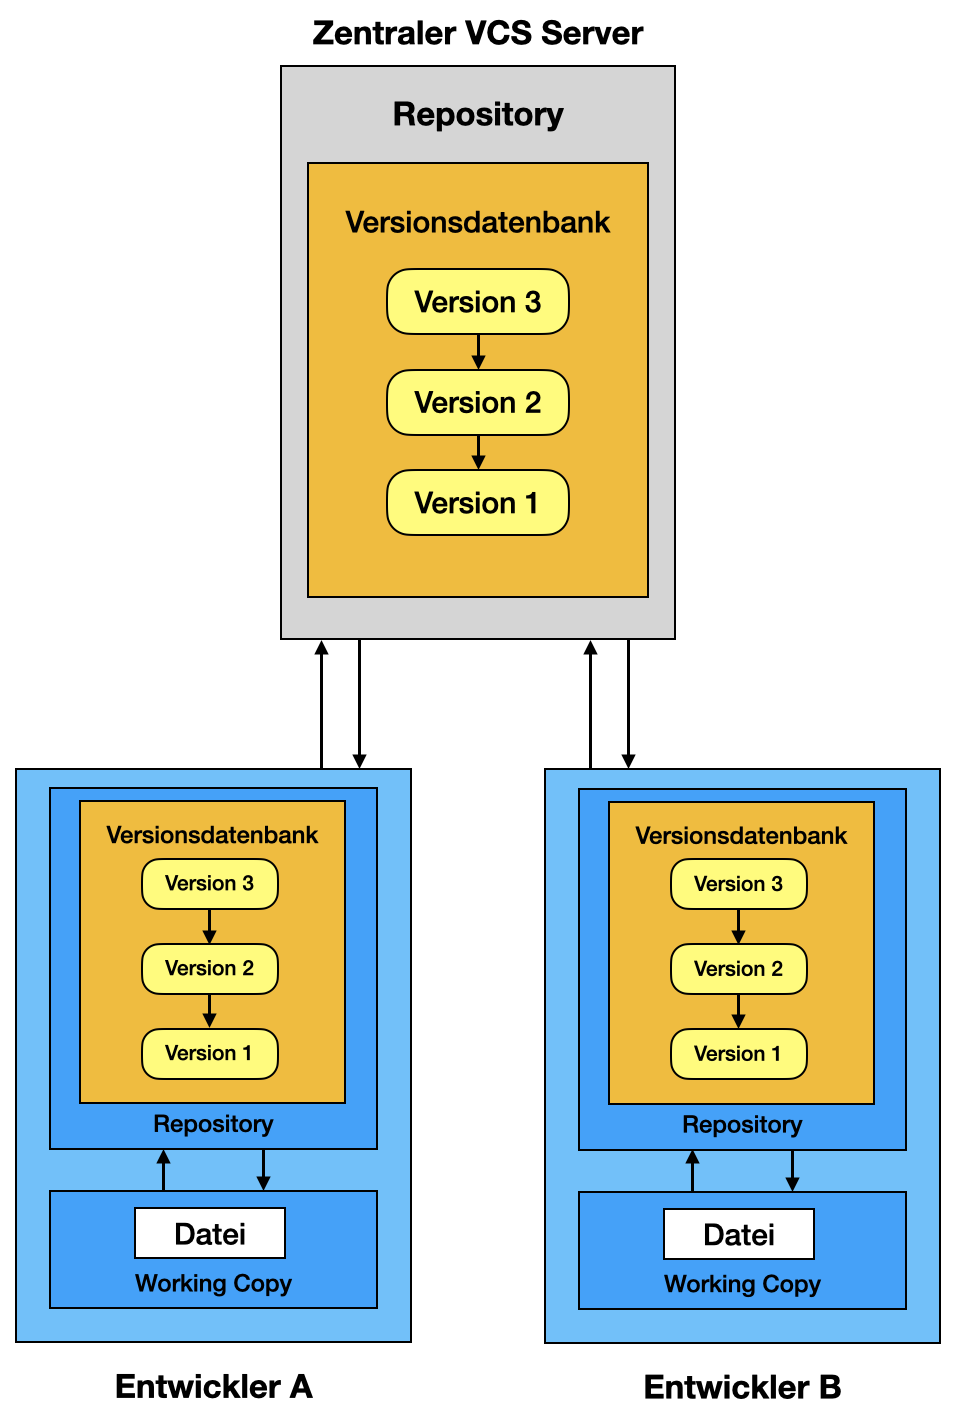
\includegraphics[scale=.6]{images/distributed_vcs.png}
	\end{center}
		\caption{Verteiltes Versionskontrollsystem}
	\end{figure}
\end{itemize}

\subsection{Git}
Git \cite{git_2020} ist ein Open-Source-Tool, das von Linus Torvalds, dem Entwickler des Betriebssystems Linux, entwickelt wurde und stammt aus dem Jahr 2005. Heutzutage zählt es zu eines der weitverbreitesten Versionsverwaltungssysteme weltweit. Die Softwareentwickler kommen sowohl aus dem kommerziellen als auch aus dem öffentlichen Bereich. Aufgrund seiner Architektur ist Git ein Distributed VCS (DVCS, dt. verteiltes VCS) und funktioniert in zahlreichen Plattformen und Entwicklungsumgebungen. Das bedeutet, dass auf die gesamte History mit allen Entwicklungsarbeiten von jedem Standort aus zugegriffen werden kann. Neben seinem verteilten System ist Git unter anderem auf Performance, Sicherheit und Flexibilität fokussiert.

\paragraph{Snapshots}\mbox{}\\
Bei den meisten VCS werden Informationen als eine Liste mit den Änderungen innerhalb der Dateien gespeichert. Das bedeutet, dass bei jeder Version nur die Dateien festgehalten werden, deren Inhalt sich während den Entwicklungsarbeiten geändert haben.

\begin{figure}[H]
\begin{center}
	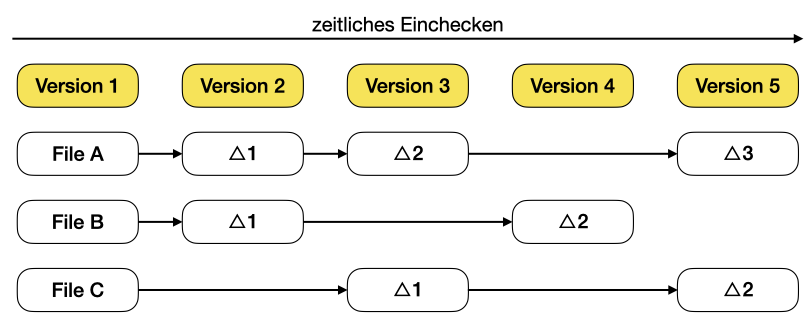
\includegraphics[scale=.4]{images/other_vcs.png}
\end{center}
	\caption{Speichern von Daten bei anderen VCS}
\end{figure} 

\mbox{}\\Im Gegensatz dazu werden die Daten als eine Art Folge von Schnappschüssen (engl. snapshots) betrachtet. Nach jedem Commit wird der aktuelle Stand des Repositories gespeichert. Dieser beinhaltet die gesamte Kopie des Projekts zu diesem Zeitpunkt und erhält eine Referenz zu diesem Schnappschuss in Form eines einzigartigen Hashwertes. Wenn das Entwicklerteam weiter am Projekt arbeitet und die Änderungen committet, erhalten die neuen und geänderten Dateien eine neuen Commit-Hash, während die Dateien, die sich nicht geändert haben, nur auf dieselbe Datei im vorherigen Schnappschuss verlinkt werden.

\begin{figure}[H]
\begin{center}
	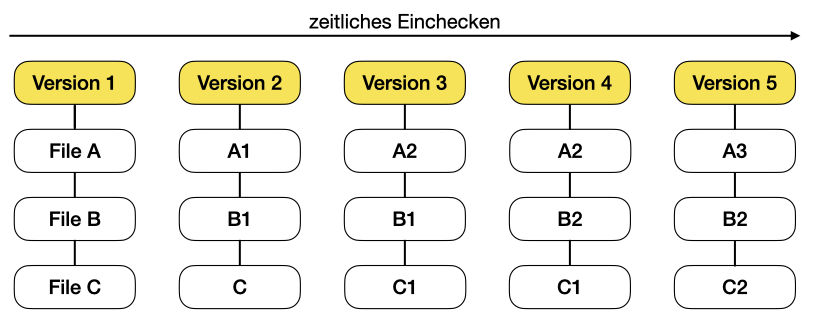
\includegraphics[scale=.4]{images/git_snapshot.png}
\end{center}
	\caption{Speichern von Daten bei Git}
\end{figure}

\mbox{}\\Um eine Sicherheit garantieren zu können, werden die Dateiinhalte sowie ihre Beziehungen zu anderen Dateien, Verzeichnissen, Versionen, Commits und Tags mit dem Hashing-Algorithmus SHA1 gesichert. Dadurch kann der Quellcode des Entwicklers vor ungewollten Änderungen geschützt und die Historie vollständig mitverfolgt werden. In der Datenbank werden keine Dateinamen sondern nur Hashwerte gespeichert. Ein Beispiel für so einen Wert ist \texttt{fe215ed7198155ca796fbb8ef81683137c210492}.\\

\paragraph{Workflow}\mbox{}\\
In einem Git-Projekt sind die drei wichtigsten Stufen das Working Directory, die Staging Area und das Repository, wobei dieses in das \texttt{local} und das  \texttt{remote} Repository gegliedert werden kann. Mit  \texttt{add} wird eine Kopie des Working Directory erstellt, wobei die Änderungen an den Dateien mit  \texttt{new},  \texttt{modified} oder  \texttt{deleted} gekennzeichnet sind. Die Arbeitskopie befindet sich nun in der Staging Area und noch nicht in der Datenbank. Nun haben die Dateien den Status  \texttt{staged} und können im nächsten Schnappschuss eingepflegt werden. Nach einem  \texttt{commit} wird ein Schnappschuss im lokalen Repository erstellt, der mit einem  \texttt{push} in der Datenbank und somit im entfernten Repository gesichert wird.

\begin{figure}[H]
\begin{center}
	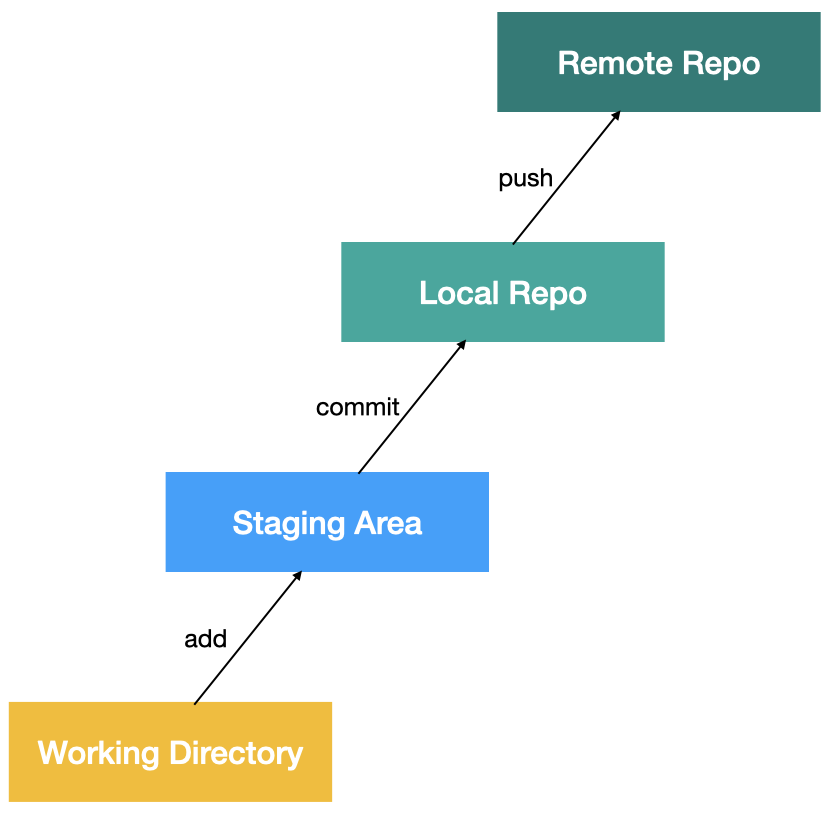
\includegraphics[scale=.3]{images/git_workflow.png}
\end{center}
	\caption{Die drei Hauptstufen von Git}
\end{figure}

\paragraph{Merge}\mbox{}\\
Oftmals werden Entwicklungszweige erstellt um Bugs zu beheben oder an neuen Funktionalitäten einer Software zu arbeiten. Diese Änderungen sollen zu einem späteren Zeitpunkt in einen einzigen Branch integriert werden, der in den meisten Fällen der Hauptzweig \texttt{master} ist. Dies wird durch einen Merge ermöglicht.

 \mbox{}\\
Mehrere Commits aus zwei Entwicklungszweigen werden in einen einheitlichen Verlauf zusammengeführt und die Branches somit vereint. Im Prinzip sucht sich der Pointer der Commits einen gemeinsamen Commit als Basis des Merges. Genau dann, wenn diese Basis gefunden wird, wird ein zusätzlicher Commit für den Merge erstellt. Dadurch werden alle seither vorgenommenen Änderungen in einen gemeinsamen Verlauf vereint.

\begin{figure}[H]
\begin{center}
	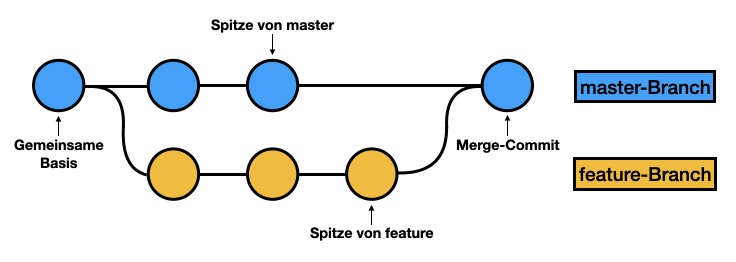
\includegraphics[scale=.8]{images/git-merge.png}
\end{center}
	\caption{Mergen von zwei Branches mit Merge-Commit}
\end{figure}

 \mbox{}\\
Im Gegensatz zu einfachen Commits während der Entwicklung, haben Merge-Commits zwei übergeordnete Commits. Sind Änderungen in beiden Branches vorgenommen worden, können von Git nicht automatisch zusammengeführt werden. Dies führt oftmals zu einem Merge-Konflikt, der von dem Entwickler manuell beseitigt werden muss. Im Normalfall kann Git die Commit-Historie automatischen zusammenführen, es sei denn es gibt Änderungen im aktuellen Branch und im Ziel-Branch, die zu Konflikten im Projekt führen.

 \mbox{}\\
Grundsätzlich gibt es zwei Arten von Merges:

\begin{itemize}
	\item \textbf{Fast-Forward-Merge:}\\
		Wenn der Verlauf vom aktuellen Entwicklungszweig zum Ziel-Branch linear ist, findet ein Fast-Forward-Merge
		statt. Linear bedeutet, dass nur an einem Entwicklungszweig Änderungen vorgenommen worden sind und der 
		andere genauso geblieben ist, wie zu dem Zeitpunkt, an dem der andere Branch erstellt worden ist.\\
		Bei diesem Merge wird ausschließlich der Pointer des Ziel-Branches auf die Commit-Spitze des aktuellen 
		Branches gelegt. Somit werden die beiden Entwicklungszweige kombiniert und enthalten dieselbe 
		Commit-Historie. Da lediglich die Position des Pointers verändert wird, erstellt Git keinen Merge-Commit. 
		Für den Fall, dass kein linearer Pfad zum Ziel-Branch existiert, erfolgt das Zusammenführen der Branches
		mit einem 3-Way-Merge. 
		
		\begin{figure}[H]
		\begin{center}
			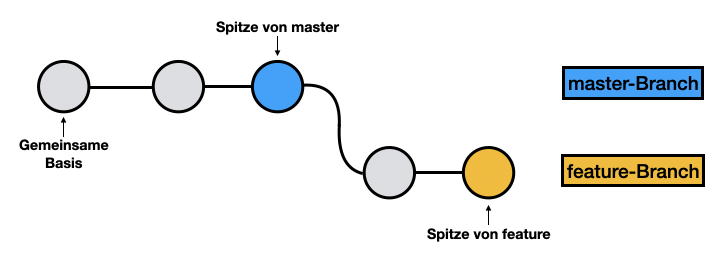
\includegraphics[scale=.8]{images/git-fast-forward-merge-before.png}
		\end{center}
			\caption{Es werden Änderungen am \texttt{feature}-Branch vorgenommen, der \texttt{master}-Branch
				bleibt gleich.}
		\end{figure}
		
		\begin{figure}[H]
		\begin{center}
			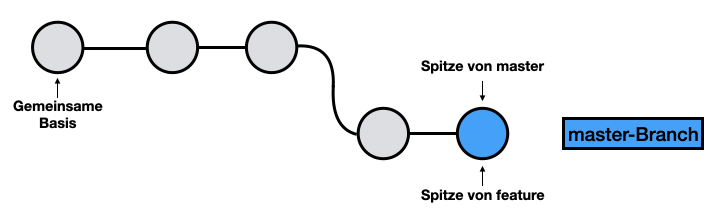
\includegraphics[scale=.8]{images/git-fast-forward-merge-after.png}
		\end{center}
			\caption{Die Änderungen des \texttt{feature}-Branches werden in den \texttt{master}-Branch eingepflegt.}
		\end{figure}
		
	\item \textbf{3-Way-Merge:}\\
		Die Bezeichnung 3-Way-Merge kommt daher, dass für das Zusammenführen von zwei Entwicklungszweigen 
		drei Commits benötigt werden. Zwei Commits sind die Spitzen der beiden Branches und ein Commit ist ihr
		gemeinsamer Basis-Commit.\\
		Hierbei werden seit der Erstellung eines neuen Entwicklungszweiges sowohl 
		am Ziel-Branch als auch am aktuellen Branch neue Änderungen gemacht, die wieder zusammengeführt
		werden sollen. Vor allem beim Entwickeln neuer umfangreicher Funktionalitäten oder beim zeitgleichen 
		Arbeiten am selben Projekt mit mehreren Entwicklern, ist ein 3-Way-Merge erforderlich. \\
		Allerdings kann es hierbei zu Konflikten während eines Merges kommen, die von dem Entwickler selbst
		gelöst werden muss.
		
		\begin{figure}[H]
		\begin{center}
			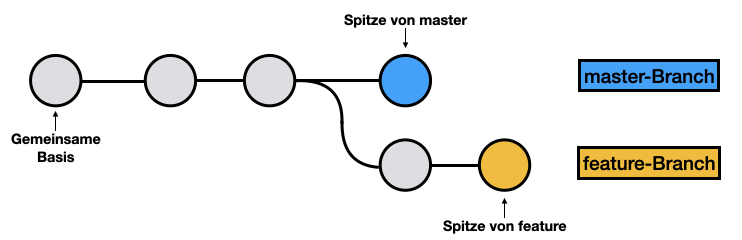
\includegraphics[scale=.8]{images/git-3-way-merge-before.png}
		\end{center}
			\caption{Es werden Änderungen am \texttt{feature}-Branch am \texttt{master}-Branch vorgenommen.}
		\end{figure}
		
		\begin{figure}[H]
		\begin{center}
			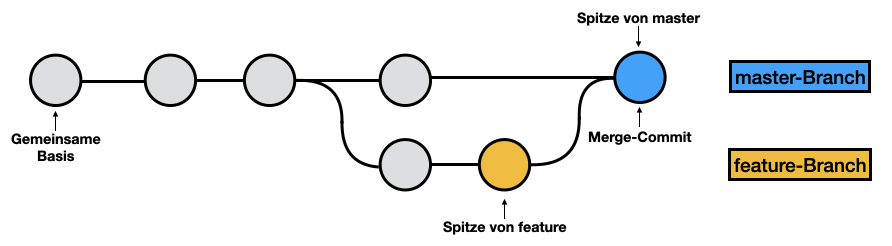
\includegraphics[scale=.8]{images/git-3-way-merge-after.png}
		\end{center}
			\caption{Die Änderungen des \texttt{feature}-Branches werden mit einem Merge-Commit in den 
				\texttt{master}-Branch eingepflegt.}
		\end{figure}
\end{itemize}

\subsection{GitLab}
Im Jahr 2011 wurde GitLab \cite{gitlab_2020} von den ukrainischen Entwicklern Dmitri Saparoschez und Valery Sizov ursprünglich in der Programmiersprache Ruby on Rails und mittlerweile noch zusätzlich in Go und Vue.js geschrieben. Es ist eine Webapplikation zur Versionskontrolle, das auf Git basiert. Neben dem Arbeiten mit Git stellt diese Anwendung einige weitere Funktionen zur Verfügung. Diese sind beispielsweise eine integrierte und kostenlose Continuous Integration/Delivery (CI/CD), das Issue Tracking, die Wiki-Funktion und vieles mehr. Zusätzlich können Rollen zugewiesen werden, die die Berechtigungen von den jeweiligen Nutzern festlegen.

\mbox{}\\Seit 2013 gibt es zwei Linzenzmodelle von GitLab. Die Community Edition (CE) wird unter der MIT-Lizenz als Open-Source-Software entwickelt und ist auf gitlab.com als Software as a Service (SaaS) erreichbar. Hingegen wird die Enterprise Edition unter einer proprietären Lizenz entwickelt und beinhaltet mehr Funktionen, die für Unternehmen relevanter sind.

\section{Hypertext Markup Language}
Hypertext Markup Language, kurz HTML \cite{html_2021}, ist eine Auszeichnungssprache, welche den Inhalt und die Struktur einer Webseite definiert. Die Strukturierung kann dabei in Paragraphen, Listen, Bildern, Tabellen und einigen anderen Elemente erfolgen. 

\mbox{}\\
\textbf{''Hypertext''} bezeichnet die Links, die entweder auf HTML-Elemente innerhalb einer Webseite verlinkt oder mehrere Webseiten miteinander verbindet. Grundsätzlich werden mithilfe von Links Inhalte in das Internet hochgeladen und mit Seiten verlinkt.\\
\textbf{''Markup''} dient dazu Texte, Bilder sowie weitere Inhalte zur Darstellung in einem Webbrowser zu annotieren.\\
Ein HTML-Element wird in den sogenannten \textbf{''Tags''} auf einer Webseite platziert. Dabei wird der Name des Elementes zwischen die Klammern \texttt{<} und \texttt{>} gegeben. Diese Tags sind case-insensitive, weshalb sie in Groß- oder Kleinbuchstaben oder in einer Mischung dieser geschrieben werden können. Beispielsweise kann ein \texttt{<label>} Tag auch als \texttt{<LABEL>} oder \texttt{<Label>} definiert werden.

\mbox{}\\
Zusätzlich zu HTML kommen andere Technologien wie Cascading Style Sheets, auch CSS, und JavaScript zum Einsatz. Dabei beschreibt CSS das Aussehen der Webseite während JavaScript die Funktionalität und das Verhalten festlegt. 

\subsection{HTML-Elemente}

\paragraph{Aufbau}

\mbox{}\\
Ein HTML-Element ist vorwiegend zusammengesetzt aus einem öffnenden und einem schließenden Tag sowie der Inhalt zwischen diesen Tags. Es ist eine Art Container oder Behälter für die Informationen, die innerhalb von ihm definiert sind.

\begin{figure}[H]
	\begin{center}
		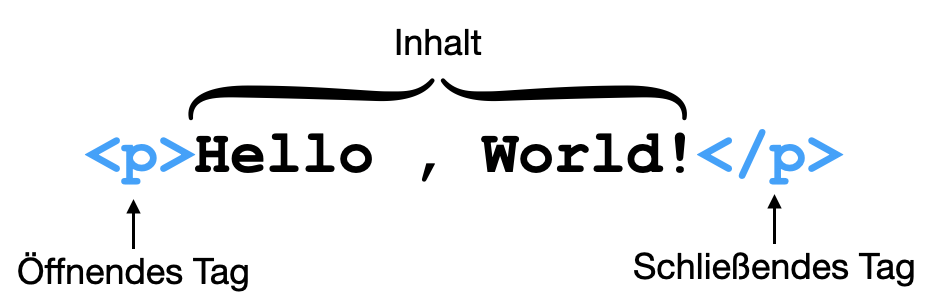
\includegraphics[scale=.6]{images/html-element-example.png}
	\end{center}
		\caption{Beispiel eines HTML-Elementes}
\end{figure}

\begin{itemize}
	\item Das \textbf{öffnende Tag} ist zusammengesetzt aus spitzen Klammern \texttt{< >}, die den Namen des 
		HTML-Elementes 
		umschließen. Es gibt die Stelle an, an der das Element beginnt.
	\item Das \textbf{schließende Tag} ist ähnlich dem öffnenden Tag nur, dass zusätzlich ein Schrägstrich \texttt{/} vor dem
		Namen des HTML-Elementes steht. Es gibt die Stelle an, an der das Element endet. 
	\item Der \textbf{Inhalt} des HTML-Elementes steht zwischen diesen beiden Tags. In der Abbildung handelt es sich hierbei 
		um einen simplen Text.
\end{itemize}

\mbox{}\\
Des Weiteren können HTML-Elemente Attribute beinhalten, die in den spitzen Klammern und nach dem Namen des öffnenden Tags geschrieben werden. Attribute geben Auskunft über zusätzliche Informationen über das Element, der nicht im Inhalt ersichtlich sein soll. Dabei müssen folgende Voraussetzungen erfüllt sein:

\begin{itemize}
	\item Zwischen dem HTML-Elementname und dem Attribut oder mehreren Attributen muss ein Leerzeichen sein.
	\item Nach dem Attributnamen folgt ein Gleichheitszeichen \texttt{=}.
	\item Der Attributwert muss von Anführungszeichen \texttt{"} umschlossen sein.
\end{itemize}

\paragraph{Verschachtelte Elemente}
\mbox{}\\
HTML-Elemente, die sich innerhalb eines Elementes befinden, werden als Verschachtelung bezeichnet. Dabei muss stets darauf geachtet werden, dass die Tags wieder korrekt geschlossen werden. Befindet sich zum Beispiel ein \texttt{<strong>} Tag innerhalb eines \texttt{<p>} Tag, muss darauf geachtet werden, dass der innere Tag vor dem äußeren Tag geschlossen wird. 

\paragraph{Leere Elemente}
\mbox{}\\
Obwohl die meisten HTML-Elemente einen Inhalt haben, gibt es dennoch einige, die keinen besitzen. Dazu zählt beispielsweise der \texttt{<img>} Tag. Bei diesem Element gibt es keinen schließenden Tag und es umhüllt auch keinen Inhalt. Der Zweck hinter
diesen Tags ist es, einzelne Gestaltungselemente einzubinden.

\begin{figure}[H]
	\begin{center}
		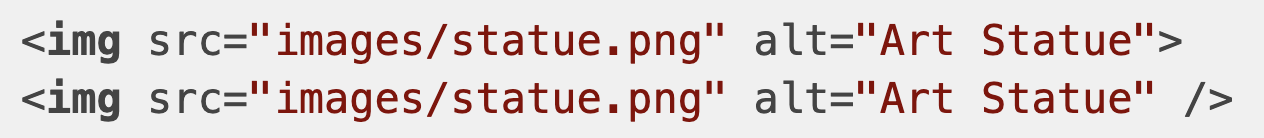
\includegraphics[scale=.5]{images/empty-element-example.png}
	\end{center}
		\caption{Beispiel eines leeren HTML-Elementes}
\end{figure}

\mbox{}\\
Damals ist mit Extensible HTML, kurz XHTML am Ende eines leeren HTML-Tags ein Schrägstrich gesetzt worden. Mit HTML5 kann dieser weggelassen werden. 

\subsection{Aufbau eines HTML-Dokumentes}

\begin{figure}[H]
	\begin{center}
		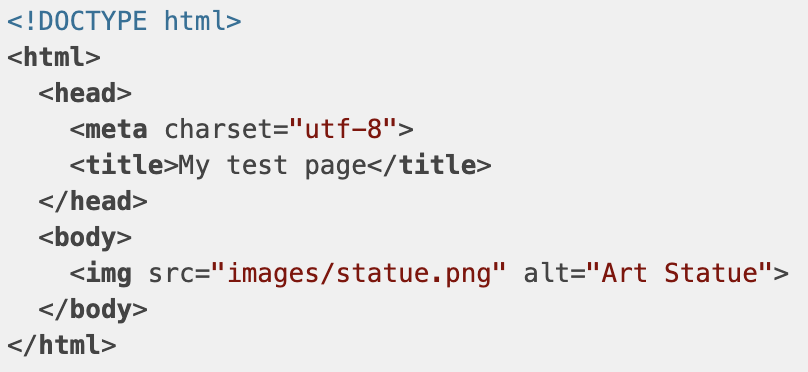
\includegraphics[scale=.7]{images/html-document-structure.png}
	\end{center}
		\caption{Aufbau eines HTML-Dokumentes}
\end{figure}

Die folgenden HTML-Tags bilden zusammen eine HTML-Seite:

\begin{table}[H]
	\begin{center}
	\begin{tabular}{| c | m{10cm} |}
		\hline
 		\cellcolor{Gray}\textcolor{White}{HTML-Element} & \cellcolor{Gray}\textcolor{White}{Beschreibung}  \\
		\hline
		\texttt{<!DOCTYPE html>} & Damals hat dieses Tag dazu gedient, um mit Prüfung von Fehlern und anderen 
			Überprüfungen sicherzustellen, dass die HTML-Seite gut dargestellt wird und funktioniert. Heute dient dieses Tag 
			lediglich dazu, um sicherzugehen, dass das Verhalten des Dokumentes korrekt ist.\\
		\hline
		\texttt{<html></html>} & Diese Element schließt den gesamten Inhalt einer HTML-Seite ein und wird auch als Root-
			Element bezeichnet.\\
		\hline
		\texttt{<head></head>} & Dieses Element ist eine Art Container und umfasst alles, was auf der Webseite beinhaltet, 
			aber nicht für den Betrachter sichtbar sein soll. Dazu zählen zum Beispiel Gestaltungen mit CSS, 
			Zeichensatzdeklarationen und vieles mehr.\\
		\hline
		\texttt{<title></title>} & Damit wird der Titel der Webseite beschrieben, der in der Registerkarte des Browsers angezeigt 
			wird.\\
		\hline
		\texttt{<body></body>} & Dieser HTML-Tag beinhaltet den Inhalt, der für die Benutzer der Webseite angezeigt wird. \\
		\hline
	\end{tabular}
	\end{center}
	\caption{Unterstützte Funktionalitäten der Tastatur}
\end{table}

\newpage
\section{JavaScript}
JavaScript, kurz JS~\cite{javascript_2021} , basiert auf dem ECMAScript Standard und ist eine dynamische, funktionale und objektorientierte Skriptsprache, die im Mai 1995 innerhalb von 10 Tagen von Brendan Eich entwickelt worden ist. Erstmals ist sie bei Netscape für dynamisches HTML in Webbrowsern zum Einsatz gekommen. Mittlerweile wird JS auch auf Servern oder Mikrocontrollern verwendet.

\subsection{ECMAScript}
ECMAScript~\cite{ecma_262_2020} gibt vor welche JavaScript Funktionalitäten von Webbrowsern implementiert werden müssen. Somit kann erreicht werden, dass Webseiten ohne Bedenken in jedem beliebigen Browser funktionsfähig sind. Gäbe es diesen Standard nicht, müssten Polyfills eingesetzt werden. Diese würden Funktionalitäten in JavaScript implementieren, die jeder Browser verstehen sollte. Diese Notlösung führt dazu, dass zusätzlich mehr programmiert wird, der Nutzer viel größere Dateien herunterladet, die Lösung nicht nativ ist und die Performance darunter leidet. 

\subsection{Dynamische Typisierung}
JavaScript ist schwach typisierte und dynamische Programmiersprache. Wenn Variablen erstellt werden, haben sie keinen expliziten Datentyp. Anhand des Wertes einer Variable ändert sich intern auch ihr Datentyp. Der aktuellste ECMAScript Standard definiert neun Typen, die in zwei Kategorien unterteilt werden können.

\paragraph{Primitive Datentypen:}

\begin{itemize}
	\item \texttt{undefined}: Die Variable hat keinen Datentyp oder wurde explizit als \texttt{undefined} angegeben.
	\item \texttt{Boolean} ist ein logischer Datentyp der einen Wahrheitswert  \texttt{true} oder  \texttt{false} annehmen 	
		kann.
	\item \texttt{Number} ist ein numerischer Datentyp, der dem IEEE 754 konform ist. Das heißt, dass fast alle Zahlen, 
		inklusive ganze Zahlen als Gleitkommazahl gespeichert werden.
	\item \texttt{String} ist eine Sequenz von Buchstaben.
	\item \texttt{BigInt} ist ein numerischer Datentyp, der ganze Zahlen in der Langzahlarithmetik darstellt.
	\item \texttt{Symbol} ist ein eindeutiger String, der nicht mehrmals erstellt werden kann. Es wird als Objekteigenschaft 
		verwendet. Somit können JavaScript-Objekte wiederholt denselben Eigenschaftsnamen verwenden.
	\item \texttt{null} gibt an, das absichtlich ein Wert fehlt und die Variable auf kein Objekt zeigt.
\end{itemize}

\paragraph{Strukturierte Typen:}

\begin{itemize}
	\item \texttt{Object}: Alle Variablen, die mit  \texttt{new} angelegt werden, sind Objekte. Dazu zählt auch das 
		JavaScript-Objekt \texttt{\{ ... \}}.
	\item \texttt{Function} gibt den Datentypen an, die als JavaScript-Funktion mit dem Schlüssenwort \texttt{function}
		deklariert worden ist.
\end{itemize}

\paragraph{Unterschied zwischen \texttt{==} und \texttt{===}}

\mbox{}\\
\texttt{==} überprüft auf Gleichheit der beiden Variablen. Sollten diese nicht vom gleichen Typ sein, werden diese auf denselben Datentyp konvertiert. Referenzen gelten gleich, wenn sie auf dasselbe Objekt zeigen.

\begin{itemize}
	\item \texttt{1 == 1}
	\item \texttt{'1'== 1}
	\item \texttt{1 == true}
	\item \texttt{0 == false}
\end{itemize}

\mbox{}\\
\texttt{===} achtet genauso wie oben genannt auf den Inhalt mit dem Unterschied, dass davor überprüft wird, ob beide Variablen denselben Typ haben.

\mbox{}\\
Dasselbe gilt für die Überprüfung der Ungleichheit \texttt{!=} und \texttt{!==}.

\section{TypeScript}

\section{Node.js und npm}

\subsection{Node.js}
Node.js (vgl.\cite{nodejs_2021}) ist eine JavaScript-Laufzeitumgebung mit der JavaScript-Code außerhalb eines Webbrowsers ausgeführt werden kann. Somit kann der Code nicht nur clientseitig, sondern auch serverseitig verwendet werden. Node.js hat eine eventbasierte Architektur und wird auf der im Jahr 2009 von Google entwickelten Open-Source-JavaScript-Engine V8 ausgeführt, der ursprünglich nur für Browser verwendet worden ist.\\
Zu den Einsatzgebieten gehören die Entwicklung von Webservern, die Erstellung von Skripten oder Tools im Terminal sowie seit neuestem die Entwicklung von Desktopanwendungen. Neben der Laufzeitumgebung stellt Node.js seine Core-API zur Verfügung. Diese reicht von simplen Netzwerkzugriffen bis hin zu Zugriffen auf Dateien.

\paragraph{Vorteile und Gründe zur Verwendung von Node.js}
\mbox{}\\
Mit seiner eventbasierten Architektur führt Node.js nur einen einzigen Thread aus, in dem ein Event Loop läuft. Im Gegensatz zu Node.js verwenden traditionelle Webframeworks für jede Anfrage auf den Server einen eigenen Thread. Näher betrachtet kann das Starten eines Threads einige Nachteile mit sich bringen. Angenommen ein Thread, der lediglich die Anfrage bearbeitet, benötigt 2 MB im Hauptspeicher, beginnt die Überlastung eines Servers mit 8 GB Hauptspeicher und 4000 gleichzeitigen Anfragen \cite{nodejs_blogpost_2012}.\\
Mit der Verwendung eines einzigen Threads, muss auch dementsprechend mit Gefahren gerechnet werden.

\mbox{}\\
Rechenintensive Anfragen könnten den einzigen Thread überlasten und alle anderen Anfragen verzögern. Diese Verlangsamung würde solange andauern bis dieser rechenintensive Prozess fertig ausgeführt worden ist. Im Normalfall wird bei einer Exception oder bei einem Fehler der Thread gestoppt. Ist allerdings nur ein einzelner Thread vorhanden, kann ein Fehler bereits zum Absturz des Programmes führen. Um das Abstürzen aufgrund von Exceptions zu vermeiden können diese Fehler mit Callbacks verarbeitet werden.

\paragraph{Konkurrenz}
\mbox{}\\
Deno (vgl. \cite{deno_2021}) ist genauso wie Node.js eine JavaScript-Laufzeitumgebung und ist von demselben Entwickler Ryan Dahl. Seiner Meinung nach hat Node.js viele Probleme gehabt und er ist auch nicht mit der Benutzerfreundlichkeit zufrieden gewesen. Aus diesem Grund ist Deno erstmals im Jahr 2018 veröffentlicht worden. Neben JavaScript wird auch TypeScript nativ unterstützt und ein großer Wert auf die Sicherheit mit Erlaubnissen gelegt. Ein Modulsystem wie npm kommt nicht mehr zum Einsatz. Externe Module beziehungsweise Bibliotheken werden mit absoluten Adressen importiert. Dieses Konzept ist von Golang inspiriert.

\subsection{npm}
\cite{npm_2021}

\section{Webpack}
Webpack~\cite{webpack_2021} ist ein statische Modul-Bundler für JavaScript-Applikationen. Mehrere JavaScript-Dateien werden zur Nutzung in einem Webbrowser zusammengeführt und zu einer oder mehreren Dateien gebündelt, abhängig von der Anzahl an Modulen. Diese Module werden intern in einem Abhängigkeitsgraphen dargestellt. Rekursiv beginnt dieser vom Eingangspunkt und fügt alle Abhängigkeiten in diesen Graphen ein. Somit wird nur der Code zusammengebündelt, der auch benötigt wird. \\
Des Weiteren kann Webpack mithilfe einer JavaScript-Datei konfiguriert werden.

\mbox{}\\
Das Konzept von Webpack kann in sechs Kernpunkte unterteilt werden:

\subsection{Entry}
Der Eingangspunkt gibt an wo Webpack beginnen soll das Bundle zusammenzusetzen. Anhand dieses Punktes kann herausgefunden werden welche Abhängigkeiten direkt oder indirekt benötigt werden, die anschließend in den Abhängigkeitsgraphen eingefügt werden. 

\begin{figure}[H]
	\begin{center}
		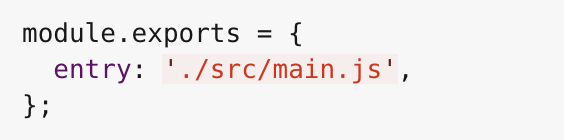
\includegraphics[scale=.7]{images/webpack-entry-point.png}
	\end{center}
		\caption{webpack.config.js}
\end{figure}

\subsection{Output}
Der Output definiert wie Webpack die zusammengebündelten benennen oder wo sie gespeichert werden sollen. 

\begin{figure}[H]
	\begin{center}
		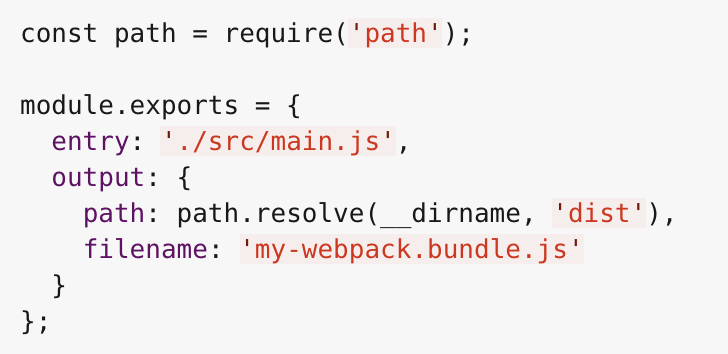
\includegraphics[scale=.7]{images/webpack-output.png}
	\end{center}
		\caption{webpack.config.js}
\end{figure}

\subsection{Loaders}
Webpack unterstützt nur JavaScript und JSON Dateien als Import im Code. Mit Loadern is es möglich Webpack so zu erweitern, dass andere Dateien ebenfalls importiert und in den Abhängigkeitsgraphen eingefügt werden können. Diese Loader besitzen zwei wichtige Eigenschaften:

\begin{enumerate}
	\item \texttt{test} gibt an welche Dateien von diesem Loader verwendet werden. Hierbei handelt es sich um einen 
		regulären Ausdruck.
	\item \texttt{use} legt fest welcher Loader beziehungsweise welche Bibliothek für die Dateien verwendet werden sollen.
\end{enumerate}

\begin{figure}[H]
	\begin{center}
		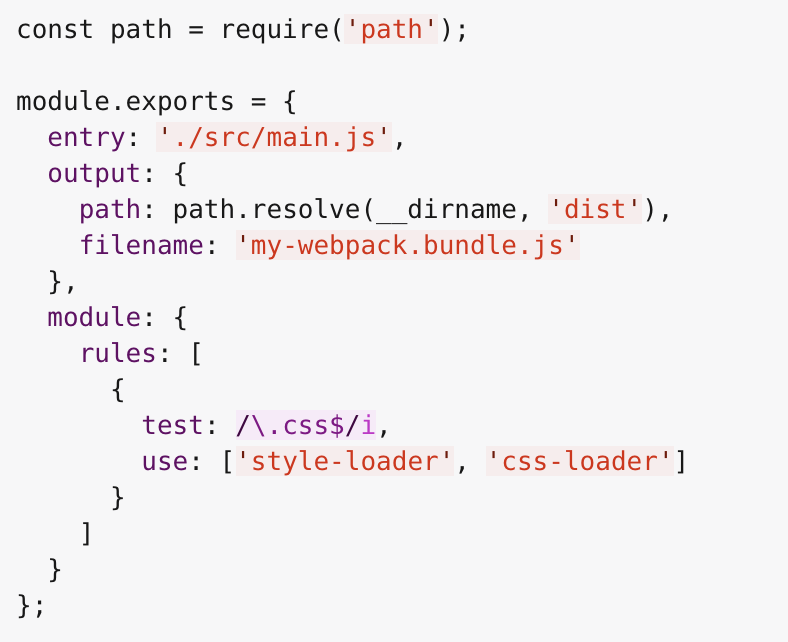
\includegraphics[scale=.7]{images/webpack-loaders.png}
	\end{center}
		\caption{webpack.config.js}
\end{figure}

\mbox{}\\
In der obigen Abbildung ist die Eigenschaft \texttt{rules} definiert mit den beiden erforderlichen Eigenschaften \texttt{test} und \texttt{use}. \texttt{rules} sagt dem Webpack Compiler, dass dieser die Dateien mit der Endung \texttt{.css} innerhalb eines \texttt{require()} oder \texttt{import} Statements mit einem \texttt{css-loader} umwandeln soll. Anschließend werden die transformierten Dateien zum Bundle hinzugefügt.

\subsection{Plugins}
Mithilfe von Plugins besteht die Möglichkeit Webpack so zu erweitern, dass gewisse Funktionalitäten optimiert, automatisiert oder neu hinzugefügt werden. Die Verwaltung von Assets und das Injizieren von Umgebungsvariablen ist ebenso möglich. 
\mbox{}\\
Plugins können verwendet werden, indem das \texttt{require()} Statement verwendet und zum \texttt{plugins}-Array hinzugefügt wird. Mittels Optionen können diese angepasst werden. Ein Plugin kann mehrmals in einer Konfiguration definiert werden, weshalb mit dem \texttt{new}-Operator eine Instanz erstellt werden muss.

\begin{figure}[H]
	\begin{center}
		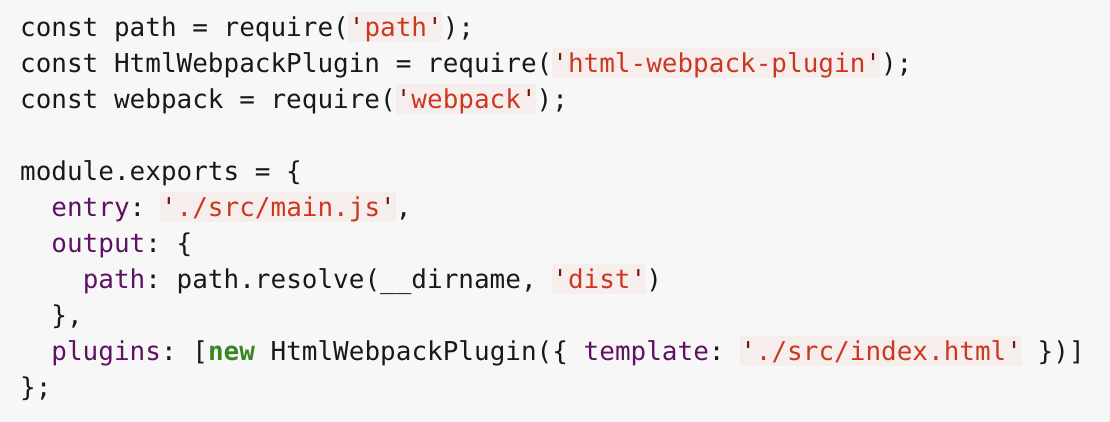
\includegraphics[scale=.7]{images/webpack-plugins.png}
	\end{center}
		\caption{webpack.config.js}
\end{figure}

\mbox{}\\
In diesem Beispiel wird das \texttt{html-webpack-plugin} verwendet, um anhand einer selbstgeschriebenen HTML-Vorlage ein Dokument zu generieren, das die JavaScript und Asset Bundles bereits importiert beziehungsweise referenziert und schließlich  im Output-Ordner \texttt{dist} ablegt.

\subsection{Mode}
Webpack gibt die Möglichkeit zu definieren in welcher Umgebung das Bundle laufen wird. Hierbei können drei verschiedene Modi gesetzt werden: \texttt{development}, \texttt{production} oder \texttt{none}. Dabei versucht Webpack intern, je nach Modus, die bestmögliche Bundle-Optimierung einzusetzen.

\begin{figure}[H]
	\begin{center}
		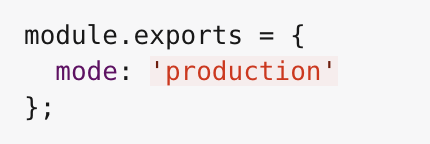
\includegraphics[scale=.7]{images/webpack-mode.png}
	\end{center}
		\caption{webpack.config.js}
\end{figure}

\subsection{Browserkompatibilität}
Es ist wichtig zu wissen, dass Webpack alle Browser unterstützt, die ES5-konform sind. Dazu zählen alle moderne und mobile Browser. Ein nichtkompatibler Webbrowser ist beispielsweise der Internet Explorer der Version 8 oder darunter. Falls diese Browser jedoch unterstützt werden sollen, wird ein Polyfill für den JavaScript Standard ES5 benötigt.











\chapter{Ausgewählte Aspekte}
\section{DOM Manipulation}

% Factory Pattern, Events, Delegate, Observer
\section{Factory Pattern}

\section{JavaScript Events \& EventListener}
\paragraph{trix-initialize}\mbox{}\\
Sobald das Trix-Editor Element im DOM eingefügt wird und sein Editor-Objekt zur Benutzung bereit ist, wird das Event \texttt{trix-initialize} gefeuert.\\
Beim Initialisieren der Toolbar wird auf das von Trix definierte Event \texttt{trix-initialize} gehört. Damit aber nicht die Standard Toolbar sondern die erweiterte Toolbar, die diese ersetzen soll, angezeigt wird, hört bei der Trix-Extension ebenso ein \texttt{EventListener} zu. Sobald das Event gefeuert wird, werden die standardmäßigen Button-Gruppen und Buttons mit denen aus der eigens erstellten Toolbar ersetzt und können mit Screenreadern und Tastaturen barrierefrei bedient werden.

\paragraph{mousedown}\mbox{}\\
Das \texttt{mousedown} Event wird genau zu dem Zeitpunkt gefeuert, an dem sich der Mauszeiger auf einem Element befindet und dieses drückt.\\
Damit ein Button in der Trix-Toolbar aktiv ist und sozusagen ``geklickt`` wird, hört dieser standardmäßig auf ein \texttt{mousedown} Event. In der Erweiterung von Trix wird dieses Event simuliert mit \texttt{EventTarget.dispatchEvent()} und somit sind die Buttons in der Toolbar auch über die Tastatur bedienbar, was vor allem bei Blinden oder bei Benutzern mit motorischen Beeinträchtigungen relevant ist.

\paragraph{keydown}\mbox{}\\
Wenn eine beliebige Taste gedrückt ist, wird das \texttt{keydown} Event gefeuert und liefert einen Code, der aussagt, welche Tasten im Moment gedrückt werden.\\
Um den WYSIWYG Texteditor mittels einer Tastatur bedienen zu können, wurde darauf gewartet bis das \texttt{keydown} Event gefeuert wurde. Je nachdem, welche Taste gedrückt wird, wird entweder der nächste oder der vorherige Button oder die Button-Gruppe fokussiert, geklickt oder der Cursor zur weiteren Texteingabe und Textformatierung in den Editor gesetzt.\\
\\Folgende Tasten und Tastenkombinationen gelten in der Toolbar und im Editor:

\begin{table}[H]
\begin{tabular}{lp{9cm}l}
\hline
Taste bzw. Tastenkombination & Beschreibung                                                                                                                                                               \\ \hline
\texttt{ALT + F10} & Befindet sich der Cursor im Editor, dann gelangt man mit dieser Tastenkombination in die Toolbar und der erste vorkommende Button wird fokussiert.                         \\ \hline
\texttt{→ oder ↓} & Der nächste bzw. rechte Button in der Toolbar wird fokussiert.                                                                                                             \\ \hline
\texttt{← oder ↑} & Der vorherige bzw. linke Button in der Toolbar wird fokussiert.                                                                                                            \\ \hline
\texttt{STRG + →/↓} & Der erste Button der nächsten bzw. rechten Gruppe wird fokussiert.                                                                                                         \\ \hline
\texttt{STRG + ←/↑} & Der erste Button der vorherigen bzw. linken Gruppe wird fokussiert.                                                                                                        \\ \hline
\texttt{ENTER oder LEERTASTE} & Der aktuell fokussierte Button wird geklickt.                                                                                                                              \\ \hline
\texttt{ESC} & Befindet sich der Fokus in der Toolbar und wird die Taste gedrückt, so wird wieder der Editor fokussiert und der Cursor befindet sich an der zuletzt verwendeten Position. 
\\ \hline
\texttt{POS1} & Der erste in der Toolbar vorkommende Button wird fokussiert.                                                                                                               \\ \hline
\texttt{ENDE} & Der letzte in der Toolbar vorkommende Button wird fokussiert.                                                                                                              \\ \hline
\end{tabular}
\end{table}

\paragraph{focusout}\mbox{}\\
Sobald ein Element im Begriff dabei ist den Fokus zu verlieren, wird das \texttt{focusout} Event gefeuert.\\
Das Dropdown Menü jedes \texttt{DropdownButtons}~\ref{dropdown_button} erhält beim Initialisieren das Attribut \texttt{hidden}, damit es zu Beginn für den Benutzer nicht sichtbar ist. Sobald der Button geklickt wird, wird auch das Menü sichtbar und der Fokus auf den ersten Button gelegt. Wenn das Menü allerdings nicht mehr fokussiert ist, reagiert der \texttt{EventListener} auf das Event \texttt{focusout} und das Dropdown Menü erhält erneut das Attribut \texttt{hidden} und wird versteckt.

\section{MutationObserver}
Der \texttt{MutationObserver} ist ein Interface, der Veränderungen in der Baumstruktur des DOMs beobachtet und wurde konzipiert, um die Mutation Events aus der DOM3 Events Spezifikation abzulösen.\\
Sobald die Toolbar geladen wird bzw. bestimmte Buttons geklickt werden, werden einige andere Buttons deaktiviert und erhalten das Attribut \texttt{disabled}. Dieses verhindert allerdings das Fokussieren eines Buttons, was mit dem Attribut \texttt{aria-disabled} problemlos funktioniert. Abhilfe verschafft deshalb ein \texttt{MutationObserver}. Erhält ein Button nun das Attribut \texttt{disabled}, beobachtet der \texttt{MutationObserver} diese Veränderung und entfernt es. Stattdessen fügt es das Attribut \texttt{aria-disabled} hinzu und setzt es auf \texttt{true}. Bei allen anderen Buttons, die nicht deaktiviert sind, ist \texttt{aria-disabled=false}.

\section{Delegation}
Die Delegation findet in der objektorientierten Programmierung verschieden Verwendung zur dynamischen Bindung von Methoden zur Programmlaufzeit.\\
Jedem \texttt{AttributeButton} kann die Identifikation eines HTML-Elements mitgegeben werden, das einen Dialog repräsentiert und bereits im HTML-Code erstellt wurde. Die Delegation ermöglicht eine Kommunikation zwischen der Trix-Toolbar und dem Dialog. Sie dient ausschließlich dazu den Dialog zu öffnen und zu schließen, wobei zwei zusätzliche Funktionalitäten das Erstellen und das Entfernen von Links sind. Alles, was während oder nach dem Dialog geschieht, wird vom Entwickler selbst bestimmt.

\section{Barrierefreie Toolbar}
% kurz beschreiben, wie Toolbar accessible wird - was macht eine accessible Toolbar aus/was machen wir
\subsection{Bedienbarkeit \& Navigation}

\subsection{Toolbar Replacer Factory}
% Baut die neue Toolbar

\subsection{Toolbar Replacer}
% Ersetzt die Toolbar

\section{Elemente der Toolbar}
\subsection{Gruppierung der Buttons}

\subsection{Button Elemente}
\label{subsec:buttons}
Es werden vier verschiedene Arten von Buttons unterschieden: 

\begin{itemize}
	\item{\textbf{Action Button}}
	\item{\textbf{Attribute Button}}
	\item{\textbf{Clickable Button}}
	\item{\textbf{Dropdown Button}}
\end{itemize}

\paragraph{Action Button}

\paragraph{Attribute Button}

\paragraph{Clickable Button}

\paragraph{Dropdown Button}
\label{dropdown_button}

\chapter{Resümee}
\section{Halil Bahar}
Mit voller Überzeugung und Motivation habe ich mein Praktikum in der Firma Fabasoft begonnen. Seit dem ersten Tag an, durfte ich viele tolle und hilfsbereite Kolleginnen und Kollegen kennenlernen, die uns bis zum Ende des Praktikums begleitet und unterstützt haben.\\
Am Anfangs des Praktikums lag der Fokus nicht am Programmieren, sondern auf der Vorbereitung für die nächsten Wochen. Wir durften an einem Workshop über Web Accessibility teilnehmen, was mir große Freude bereitet hat.

\mbox{}\\
Anschließend hat das Programmieren begonnen. In den Anfangszeiten hatten wir öfters Probleme, was die Architektur anbelangt. Wir haben lange und detailliert darüber diskutiert, welche weiteren Schritte notwendig sind. Durch diese Probleme konnte ich viele Ideen und Lösungswegen mit meinem Team besprechen und austauschen. Dieser Lernprozess hat mir besonders gut gefallen.\\
Besonders stolz war ich darauf, dass wir unsere Software rechtzeitig fertiggestellt und die letzten Wochen damit verbracht haben, unsere Software in die Fabasoft Cloud zu integrieren.


\section{Sonja Cao}
Zuversichtlich, dass wir schnell fertig werden, haben wir uns an die Arbeitsplätze gesetzt. Allerdings hat das Einarbeiten und das Aufsetzen der passenden Entwicklungsumgebungen sowie die Sammlung wichtiger Vorkenntnisse über Web Accessibility etwa eine Woche in Anspruch genommen. Nachdem dieser Schritt geschafft wurde, hat auch die tatsächliche Arbeit begonnen. \\
Mit der Unterstützung des Teams der Firma Fabasoft haben wir den besten Lösungsweg ausfindig machen können, um unser Ziel zu erreichen. Mithilfe der zahlreichen Ratschläge und Feedbacks ist es möglich gewesen Probleme schnell zu beheben, falls vorhanden, und die gewünschten Anforderungen einzupflegen. 

\mbox{}\\
Insbesondere das Ziel, einen WYSIWYG Texteditor barrierefrei zu machen, macht die Diplomarbeit zu etwas Besonderem. Dadurch können viele Menschen, unabhängig von ihrer physischen oder psychischen Einschränkungen, den Texteditor problemlos nutzen. Der Gedanke daran, dieses Ziel erreichen zu wollen, hat mich dazu motiviert, so exakt wie möglich zu arbeiten und immer mein bestes zu geben.\\
Ebenso hat mir das Auseinandersetzen mit diesem umfangreichen Thema noch viel deutlicher gemacht, dass sich viele Menschen mit Beeinträchtigungen noch benachteiligt fühlen. Es gibt noch immer zahlreiche Personen, die nicht ihr volles Potenzial entfalten können. Aus diesem Grund werde ich von nun an noch deutlicher darauf achten, dass eine barrierefreie Nutzung jeglicher Webseiten, Applikationen und sonstige Dinge wichtig ist.

\bibliography{da_bibliography}{} % end of the thesis, contains quotes etc.
\bibliographystyle{alphaurl} % alternatives plainurl, alphaurl;  german alternative: dinat (but add package natbib)

\listoffigures
\listoftables % for diagrams, drawings etc.

\appendix % attachment
\chapter{Arbeitsteilung}

\section{Halil Bahar}

\subsection{Praktische Arbeit}

\begin{itemize}
	\item Implementierung der Grundstruktur und weiterer Strukturen
	\item Qualitätssicherung
	\item Testen der Module
\end{itemize}

\subsection{Theoretische Ausarbeitung}

\paragraph{Einleitung}

\begin{itemize}
	\item Ist-Zustand
	\item Barrierefreiheit im Web
	\item Aufgabenstellung
	\item Zielsetzung
	\item Sollzustand
	\item Projektablauf und Produkt
\end{itemize}

\paragraph{Ausgewählte Technologien}

\begin{itemize}
	\item JavaScript
	\item TypeScript
	\item Node.js und npm
	\item Jest
	\item Webpack
\end{itemize}

\paragraph{Ausgewählte Aspekte}

\begin{itemize}
	\item Web Components
	\item JavaScript Events und EventListener
	\item MutationObserver
	\item Delegation
	\item Barrierefreie Toolbar
	\item Button Elemente
\end{itemize}

\section{Sonja Cao}

\subsection{Praktische Arbeit}

\begin{itemize}
	\item Implementierung weiterer Strukturen 
	\item Testen der Module
\end{itemize}

\subsection{Theoretische Ausarbeitung}

\paragraph{Einleitung}

\begin{itemize}
	\item Ausgangssituation
	\item Ist-Zustand
	\item Motivation
	\item Barrierefreiheit im Web
	\item Sollzustand
	\item Projektablauf und Produkt
\end{itemize}

\paragraph{Ausgewählte Technologien}

\begin{itemize}
	\item Git und GitLab
	\item Hypertext Markup Language
	\item TypeScript
\end{itemize}

\paragraph{Ausgewählte Aspekte}

\begin{itemize}
	\item WCAG 2.1
	\item Web Components
	\item Factory Method Pattern
	\item JavaScript Events und EventListener
	\item MutationObserver
	\item Barrierefreie Toolbar
	\item Button Elemente
\end{itemize}
\chapter{Protokolle}
\addtocontents{toc}{\protect\setcounter{tocdepth}{0}}
\section{Protokoll vom 24. Juli 2020}
\paragraph{Anwesende}
\begin{itemize}
	\item{\textbf{Prof. Thomas Stütz}}
	\item{\textbf{Halil Bahar}}
	\item{\textbf{Sonja Cao}}
\end{itemize}

\paragraph{Ort}\mbox{}\\
Sprachkonferenz über Discord

\paragraph{Inhalt}\mbox{}\\
Besprechung des Projektumfangs und der verwendeten Technologien

\section{Protokoll vom 03. August 2020}

\paragraph{Anwesende}
\begin{itemize}
	\item{\textbf{Prof. Thomas Stütz}}
	\item{\textbf{Halil Bahar}}
	\item{\textbf{Sonja Cao}}
\end{itemize}

\paragraph{Ort}\mbox{}\\
Sprachkonferenz über Discord

\paragraph{Inhalt}\mbox{}\\
Besprechung über die Erweiterung von Trix:
\begin{itemize}
	\item{Struktur des Projekts}
	\item{Verwendete Programmiersprachen sind JavaScript und TypeScript}
	\item{Bereitstellung der Barrierefreiheit}
\end{itemize}

\paragraph{Auftrag bis zum nächsten Meeting}\mbox{}\\
Erstellung einer Grafik für einen Überblick über die Schnittstellen und Beschreibung der notwendigen JavaScript Events.

\section{Protokoll vom 11. August 2020}

\paragraph{Anwesende}
\begin{itemize}
	\item{\textbf{Prof. Thomas Stütz}}
	\item{\textbf{Halil Bahar}}
	\item{\textbf{Sonja Cao}}
\end{itemize}

\paragraph{Ort}\mbox{}\\
Sprachkonferenz über Discord

\paragraph{Inhalt}\mbox{}\\
Besprechung der ersten schriftliche Ausarbeitung der Diplomarbeit:
\begin{itemize}
	\item{Bezeichnung der Kapitel}
	\item{Verbesserungsmöglichkeiten zur besseren Verständlichkeit der Arbeit}
\end{itemize}

\paragraph{Auftrag bis zum nächsten Meeting}\mbox{}\\
Verbesserung der aktuellen und Erstellung neuer Diagramme und Grafiken (Überblick über die Schnittstellen, DOM als Baumstruktur, Aussehen des Texteditors Trix) zum besseren Verständnis der Arbeit und Beginn der schriftlichen Ausarbeitung des Kapitel {\em{Einleitung}}.

\section{Protokoll vom 31. August 2020}

\paragraph{Anwesende}
\begin{itemize}
	\item{\textbf{Prof. Thomas Stütz}}
	\item{\textbf{Halil Bahar}}
	\item{\textbf{Sonja Cao}}
\end{itemize}

\paragraph{Ort}\mbox{}\\
Sprachkonferenz über Discord

\paragraph{Inhalt}\mbox{}\\
Besprechung der schriftlichen Ausarbeitung der Diplomarbeit:
\begin{itemize}
	\item{Korrigieren einzelner Rechtschreib- und Grammatikfehler}
	\item{Überlegungen über funktionale und nichtfunktionale Anforderungen}
\end{itemize}

\paragraph{Auftrag bis zum nächsten Meeting}\mbox{}\\
Beschreibung, warum der Texteditor in Fabasoft Produkten ersetzt werden muss, Verfassen kürzerer Sätze, Trennung zwischen Projektablauf und Produkt und Änderung der funktionalen und nichtfunktionalen Anforderungen.

\section{Protokoll vom 07. September 2020}

\paragraph{Anwesende}
\begin{itemize}
	\item{\textbf{Prof. Thomas Stütz}}
	\item{\textbf{Halil Bahar}}
\end{itemize}

\paragraph{Ort}\mbox{}\\
Sprachkonferenz über Discord

\paragraph{Inhalt}\mbox{}\\
Besprechung der schriftlichen Ausarbeitung der Diplomarbeit:
\begin{itemize}
	\item{Systemarchitektur mit und ohne der Erweiterung}
\end{itemize}

\paragraph{Auftrag bis zum nächsten Meeting}\mbox{}\\
Skizzieren der Systemarchitektur mit und ohne Erweiterung, Beschreibung der Zusammenhänge und Unterschiede und Verbessern der Beschreibung beim Kapitel ``Funktionale Anforderungen``.

\section{Protokoll vom 21. September 2020}

\paragraph{Anwesende}
\begin{itemize}
	\item{\textbf{Prof. Thomas Stütz}}
	\item{\textbf{Halil Bahar}}
	\item{\textbf{Sonja Cao}}
\end{itemize}

\paragraph{Ort}\mbox{}\\
Sprachkonferenz über Discord

\paragraph{Inhalt}\mbox{}\\
Besprechung der schriftlichen Ausarbeitung der Diplomarbeit:
\begin{itemize}
	\item{Kleine Grammatik- und Rechtschreibfehler}
	\item{Struktur der Kapitel}
	\item{Platzierung und Beschreibung der Systemarchitektur und des Texteditors}
\end{itemize}

\paragraph{Auftrag bis zum nächsten Meeting}\mbox{}\\
Ausbessern der Fehler, Zusätzliches Kapitel für erfüllte WCAG 2.1 Kriterien, Kapitel für Web Components

\section{Protokoll vom 09. November 2020}

\paragraph{Anwesende}
\begin{itemize}
	\item{\textbf{Prof. Thomas Stütz}}
	\item{\textbf{Halil Bahar}}
	\item{\textbf{Sonja Cao}}
\end{itemize}

\paragraph{Ort}\mbox{}\\
Sprachkonferenz über Discord

\paragraph{Inhalt}\mbox{}\\
Besprechung der schriftlichen Ausarbeitung der Diplomarbeit:
\begin{itemize}
	\item{Beschreibung der Begriffe Design Patterns und Factory Method Pattern}
	\item{Überarbeitung des Kapitels 3.5 JavaScript Events \& EventListener}
\end{itemize}

\paragraph{Auftrag bis zum nächsten Meeting}\mbox{}\\
Ergänzung des Factory Method Patterns mit einem UML-Klassendiagramm

\section{Protokoll vom 30. November 2020}

\paragraph{Anwesende}
\begin{itemize}
	\item{\textbf{Prof. Thomas Stütz}}
	\item{\textbf{Halil Bahar}}
	\item{\textbf{Sonja Cao}}
\end{itemize}

\paragraph{Ort}\mbox{}\\
Sprachkonferenz über Discord

\paragraph{Inhalt}\mbox{}\\
Besprechung der schriftlichen Ausarbeitung der Diplomarbeit:
\begin{itemize}
	\item UML-Abbildung des Factory Method Patterns: Methode \texttt{createProduct()} muss \texttt{static} sein
	\item Kapitel Git: Merging beschrieben
	\item Definieren der Arbeitsaufteilung
	\item Eventuell Beispiele für WCAG: Webseiten, die die Richtlinien erfüllen und Webseiten, die diese nicht 
		erfüllen	
\end{itemize}

\paragraph{Auftrag bis zum nächsten Meeting}\mbox{}\\
Fertigstellen aller Kapitel so weit wie möglich bis auf Kapitel Technologien

\section{Protokoll vom 14. Februar 2021}

\paragraph{Anwesende}
\begin{itemize}
	\item{\textbf{Prof. Thomas Stütz}}
	\item{\textbf{Halil Bahar}}
	\item{\textbf{Sonja Cao}}
\end{itemize}

\paragraph{Ort}\mbox{}\\
Sprachkonferenz über Discord

\paragraph{Inhalt}\mbox{}\\
Besprechung der schriftlichen Ausarbeitung der Diplomarbeit:
\begin{itemize}
	\item Fragen bezüglich Kapitel ``Verwendete Technologien``geklärt
\end{itemize}

\paragraph{Auftrag bis zum nächsten Meeting}\mbox{}\\
Beschreiben von JavaScript und TypeScript

\section{Protokoll vom 9. April 2021}

\paragraph{Anwesende}
\begin{itemize}
	\item{\textbf{Prof. Thomas Stütz}}
	\item{\textbf{Halil Bahar}}
	\item{\textbf{Sonja Cao}}
\end{itemize}

\paragraph{Ort}\mbox{}\\
Sprachkonferenz über Discord

\paragraph{Inhalt}\mbox{}\\
Besprechung der schriftlichen Ausarbeitung der Diplomarbeit:
\begin{itemize}
	\item Besprechen des Kapitels ``Verwendete Technologien``
\end{itemize}

\paragraph{Auftrag bis zum nächsten Meeting}\mbox{}\\
Beschreiben von npm, TypeScript und Webpack, Kapitel ``Ausgewählte Aspekte``ergänzen, Zitieren von Webseiten und Büchern
\end{document}  